%!TEX root = outline.tex
\begin{figure}[b!] %htb!
\centering
% This file was created by tikzplotlib v0.9.1.
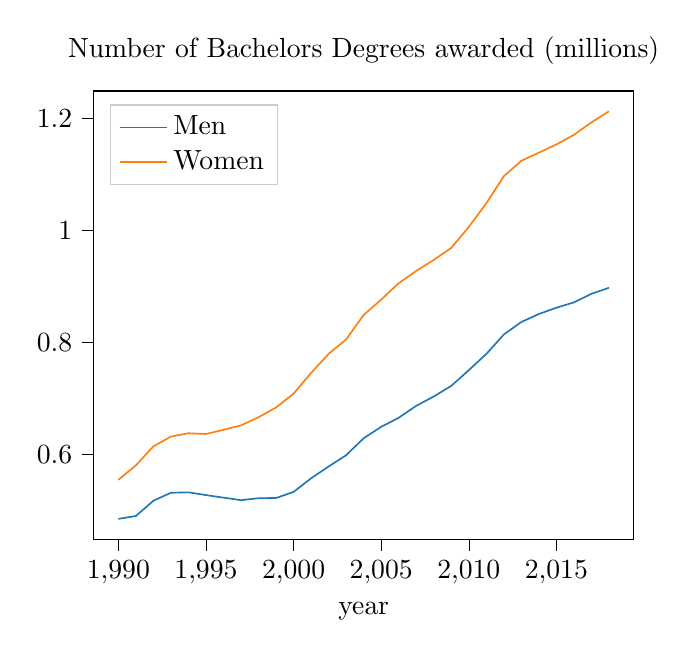
\begin{tikzpicture}

\definecolor{color0}{rgb}{0.12156862745098,0.466666666666667,0.705882352941177}
\definecolor{color1}{rgb}{1,0.498039215686275,0.0549019607843137}

\begin{axis}[
legend cell align={left},
legend style={fill opacity=0.8, draw opacity=1, text opacity=1, at={(0.03,0.97)}, anchor=north west, draw=white!80!black},
tick align=outside,
tick pos=left,
title={Number of Bachelors Degrees awarded (millions)},
x grid style={white!69.0196078431373!black},
xlabel={year},
xmin=1988.6, xmax=2019.4,
xtick style={color=black},
y grid style={white!69.0196078431373!black},
ymin=0.4493241, ymax=1.2484059,
ytick style={color=black}
]
\addplot [semithick, color0]
table {%
1990 0.48564600944519
1991 0.490826010704041
1992 0.517989993095398
1993 0.532243013381958
1994 0.532928943634033
1995 0.528069019317627
1997 0.518990993499756
1998 0.522558927536011
1999 0.522891998291016
2000 0.533735036849976
2001 0.557978987693787
2002 0.579033017158508
2003 0.599171996116638
2004 0.629392027854919
2005 0.649704933166504
2006 0.66592800617218
2007 0.687217950820923
2008 0.703808069229126
2009 0.722702980041504
2010 0.750731945037842
2011 0.779560089111328
2012 0.814333915710449
2013 0.836575031280518
2014 0.850880980491638
2015 0.862040996551514
2016 0.871549010276794
2017 0.886856079101562
2018 0.897544026374817
};
\addlegendentry{Men}
\addplot [semithick, color1]
table {%
1990 0.555091023445129
1991 0.581097006797791
1992 0.614879012107849
1993 0.632375001907349
1994 0.638270020484924
1995 0.636955976486206
1996 0.644475936889648
1997 0.652374982833862
1998 0.666815042495728
1999 0.684229016304016
2000 0.708883047103882
2001 0.745826005935669
2002 0.779849052429199
2003 0.805441975593567
2004 0.849164962768555
2005 0.87644100189209
2006 0.905745983123779
2007 0.927672982215881
2008 0.947183012962341
2009 0.968661069869995
2010 1.00603902339935
2011 1.04807901382446
2012 1.09642803668976
2013 1.12388396263123
2015 1.15306401252747
2016 1.17018795013428
2017 1.19238698482513
2018 1.2120840549469
};
\addlegendentry{Women}
\end{axis}

\end{tikzpicture}

\label{fig:n_degrees}
\end{figure}
\begin{figure}[t!] %htb!
\centering
\begin{tikzpicture}[align=left,
every node/.style={font=\footnotesize}]
% This file was created by tikzplotlib v0.9.2.
\definecolor{color0}{rgb}{0.266666666666667,0.466666666666667,0.666666666666667}
\definecolor{color1}{rgb}{0.933333333333333,0.4,0.466666666666667}
\definecolor{color2}{rgb}{0.133333333333333,0.533333333333333,0.2}
\definecolor{color3}{rgb}{0.8,0.733333333333333,0.266666666666667}
\definecolor{color4}{rgb}{0.4,0.8,0.933333333333333}
\definecolor{color5}{rgb}{0.666666666666667,0.2,0.466666666666667}

\begin{groupplot}[group style={group size=2 by 1, group name=my plots, vertical sep=2cm, horizontal sep=1.2cm}]
\nextgroupplot[
height=6.376357092455836cm,
tick align=outside,
tick pos=left,
width=9.079103cm,
x grid style={white!69.0196078431373!black},
xmin=1988.6, xmax=2030,
xtick style={color=black},
xtick={1990,1995,2000,2005,2010,2015},
xticklabels={\(\displaystyle 1990\),\(\displaystyle 1995\),\(\displaystyle 2000\),\(\displaystyle 2005\),\(\displaystyle 2010\),\(\displaystyle 2015\)},
ymajorgrids,
ymin=0, ymax=2,
ytick style={color=black},
ytick={0,0.2,0.4,0.6,0.8,1,1.2,1.4,1.6,1.8,2},
yticklabels={\(\displaystyle 0\),\(\displaystyle 0.2\),\(\displaystyle 0.4\),\(\displaystyle 0.6\),\(\displaystyle 0.8\),\(\displaystyle 1\),\(\displaystyle 1.2\),\(\displaystyle 1.4\),\(\displaystyle 1.6\),\(\displaystyle 1.8\),\(\displaystyle 2\)}
]
\addplot [semithick, color0]
table {%
1990 0.889276146888733
1991 0.908068180084229
1992 0.908786058425903
1993 0.911298394203186
1995 0.937413215637207
1996 0.960581421852112
1997 0.962796211242676
1998 0.959450006484985
1999 0.985843420028687
2000 1.00777983665466
2001 1.00261080265045
2002 1.01744496822357
2003 1.02670252323151
2004 1.02088141441345
2005 1.00308656692505
2006 0.996885895729065
2007 0.972628951072693
2008 0.96298623085022
2009 0.959978342056274
2010 0.95364236831665
2011 0.953920364379883
2012 0.931203603744507
2013 0.921860694885254
2014 0.899493217468262
2015 0.900677680969238
2016 0.891088247299194
2017 0.886778354644775
2018 0.88598895072937
};
\addplot [semithick, color1]
table {%
1990 1.22759211063385
1991 1.28919923305511
1992 1.32112109661102
1993 1.3564704656601
1994 1.39542412757874
1995 1.44826233386993
1996 1.49454152584076
1997 1.56208670139313
1998 1.59724080562592
1999 1.65807044506073
2000 1.72764885425568
2001 1.76988768577576
2002 1.76754701137543
2003 1.7330185174942
2004 1.70102310180664
2005 1.68849968910217
2006 1.65692889690399
2007 1.65950012207031
2008 1.62763059139252
2009 1.64037382602692
2010 1.63280272483826
2011 1.62376940250397
2012 1.64566314220428
2013 1.6688095331192
2014 1.67092096805573
2015 1.67829787731171
2016 1.73332345485687
2017 1.76386177539825
2018 1.79705047607422
};
\addplot [semithick, color2]
table {%
1990 0.187528491020203
1991 0.187889814376831
1992 0.18504810333252
1993 0.191165328025818
1994 0.198027372360229
1995 0.209525942802429
1996 0.219993829727173
1997 0.226323843002319
1998 0.230563402175903
1999 0.248593807220459
2000 0.259858369827271
2001 0.253314614295959
2002 0.266838073730469
2003 0.248422026634216
2004 0.258007287979126
2005 0.250089168548584
2006 0.243573904037476
2007 0.228035092353821
2008 0.227158188819885
2009 0.221451997756958
2011 0.231951236724854
2012 0.238436937332153
2013 0.240317106246948
2014 0.248236060142517
2015 0.251599311828613
2016 0.265729546546936
2017 0.274784326553345
2018 0.286244869232178
};
\addplot [semithick, color3]
table {%
1990 1.04078304767609
1991 1.04256737232208
1992 1.07366561889648
1993 1.06894600391388
1994 1.05757308006287
1995 1.10440194606781
1996 1.11996006965637
1997 1.17428719997406
1998 1.23312425613403
1999 1.30454993247986
2000 1.40134906768799
2001 1.46844744682312
2002 1.54577028751373
2003 1.63139522075653
2004 1.64863216876984
2005 1.63168549537659
2006 1.602987408638
2007 1.51491057872772
2008 1.47168242931366
2009 1.46346211433411
2010 1.41208970546722
2011 1.44205784797668
2012 1.42999362945557
2013 1.42106962203979
2014 1.41722071170807
2015 1.44253933429718
2016 1.49894797801971
2017 1.56678104400635
2018 1.64683747291565
};
\addplot [semithick, color4]
table {%
1990 0.429780006408691
1991 0.419558525085449
1993 0.395862579345703
1994 0.4017493724823
1995 0.399999976158142
1996 0.381898045539856
1997 0.373727560043335
1998 0.368845701217651
1999 0.373373627662659
2000 0.390813827514648
2002 0.384417414665222
2003 0.37157928943634
2004 0.335911631584167
2005 0.288139462471008
2006 0.261456251144409
2007 0.22909951210022
2008 0.216255187988281
2009 0.219069957733154
2010 0.223915338516235
2011 0.216599345207214
2012 0.225852251052856
2013 0.219969153404236
2014 0.223478555679321
2015 0.222921013832092
2016 0.235600471496582
2017 0.242461562156677
2018 0.257417798042297
};
\addplot [semithick, color5]
table {%
1990 0.460548996925354
1991 0.464974999427795
1992 0.4886314868927
1993 0.488829135894775
1994 0.512030601501465
1995 0.540966749191284
1996 0.565948724746704
1997 0.602615833282471
1998 0.629949331283569
1999 0.666009306907654
2000 0.686820149421692
2001 0.706353425979614
2002 0.736422896385193
2003 0.7142094373703
2004 0.72872519493103
2005 0.739134073257446
2006 0.725082635879517
2007 0.690871238708496
2008 0.687974691390991
2009 0.686181664466858
2010 0.688009262084961
2011 0.668954968452454
2012 0.67028284072876
2013 0.634251594543457
2014 0.645684003829956
2015 0.62436580657959
2016 0.629948854446411
2017 0.653665065765381
2018 0.67027759552002
};
\addplot [semithick, white!73.3333333333333!black]
table {%
1990 0.86025857925415
1991 0.899104356765747
1992 0.886856079101562
1993 0.900158047676086
1994 0.865336656570435
1995 0.88508152961731
1996 0.85411524772644
1997 0.864051580429077
1998 0.88809061050415
1999 0.93377161026001
2000 0.914776563644409
2001 0.881730198860168
2003 0.793915510177612
2004 0.801473140716553
2005 0.769950985908508
2006 0.776896238327026
2007 0.747289896011353
2008 0.764146089553833
2009 0.725896239280701
2010 0.73568868637085
2011 0.726636171340942
2012 0.726435899734497
2013 0.727647542953491
2014 0.723636150360107
2015 0.720515251159668
2016 0.709809184074402
2017 0.696071982383728
2018 0.709341764450073
};
\addplot [semithick, black]
table {%
1990 1.14299511909485
1991 1.18391644954681
1992 1.18704795837402
1993 1.18813216686249
1994 1.19766426086426
1995 1.2061984539032
1996 1.23111665248871
1997 1.25700640678406
1998 1.2760568857193
1999 1.30854749679565
2000 1.32815539836884
2001 1.33665609359741
2002 1.34681272506714
2003 1.34425842761993
2004 1.34918296337128
2005 1.3489830493927
2006 1.36012601852417
2007 1.34989619255066
2008 1.34579741954803
2009 1.34033071994781
2010 1.34007740020752
2011 1.34444940090179
2012 1.34641063213348
2013 1.34343481063843
2014 1.33796620368958
2015 1.33759760856628
2016 1.34265315532684
2017 1.34451031684875
2018 1.35044527053833
};
\draw (axis cs:2018.5,0.835989010989011) node[
  anchor=base west,
  text=color0,
  rotate=0.0
]{Business};
\draw (axis cs:2018.5,1.74705042050622) node[
  anchor=base west,
  text=color1,
  rotate=0.0
]{Social \\ Sciences};
\draw (axis cs:2018.5,0.286244813278008) node[
  anchor=base west,
  text=color2,
  rotate=0.0
]{Engineering};
\draw (axis cs:2018.5,1.44683752645192) node[
  anchor=base west,
  text=color3,
  rotate=0.0
]{Biological \\ Sciences};
\draw (axis cs:2018.5,0.037417838961352) node[
  anchor=base west,
  text=color4,
  rotate=0.0
]{Computer \\ Services};
\draw (axis cs:2018.5,0.44027762382224) node[
  anchor=base west,
  text=color5,
  rotate=0.0
]{Physical \\ Sciences};
\draw (axis cs:2018.5,0.709341764874964) node[
  anchor=base west,
  text=white!73.3333333333333!black,
  rotate=0.0
]{Math};
\draw (axis cs:2018.5,1.30044521494211) node[
  anchor=base west,
  text=black,
  rotate=0.0
]{All Fields};

\nextgroupplot[
height=6.376357092455836cm,
tick align=outside,
tick pos=left,
width=9.079103cm,
x grid style={white!69.0196078431373!black},
xmin=1988.6, xmax=2030,
xtick style={color=black},
xtick={1990,1995,2000,2005,2010,2015},
xticklabels={\(\displaystyle 1990\),\(\displaystyle 1995\),\(\displaystyle 2000\),\(\displaystyle 2005\),\(\displaystyle 2010\),\(\displaystyle 2015\)},
ymajorgrids,
ymin=0, ymax=4,
ytick style={color=black},
ytick={0,0.5,1,1.5,2,2.5,3,3.5,4},
yticklabels={\(\displaystyle 0\),\(\displaystyle 0.5\),\(\displaystyle 1\),\(\displaystyle 1.5\),\(\displaystyle 2\),\(\displaystyle 2.5\),\(\displaystyle 3\),\(\displaystyle 3.5\),\(\displaystyle 4\)}
]
\addplot [semithick, color0]
table {%
1990 2.5175244808197
1991 2.6520824432373
1992 2.74022936820984
1993 2.7347571849823
1994 2.72362613677979
1995 2.69927859306335
1996 2.70083546638489
1997 2.83463954925537
1998 2.9113347530365
1999 3.01813840866089
2000 3.2591769695282
2001 3.43097972869873
2002 3.43798732757568
2003 3.46344590187073
2004 3.48158049583435
2005 3.48040509223938
2006 3.40909743309021
2007 3.41750979423523
2008 3.35590291023254
2009 3.38099837303162
2010 3.34576916694641
2011 3.32759737968445
2012 3.26378393173218
2013 3.256920337677
2014 3.28145527839661
2015 3.37682676315308
2016 3.45335793495178
2017 3.56493353843689
2018 3.73112607002258
};
\addplot [semithick, color1]
table {%
1990 0.453454494476318
1991 0.434512615203857
1992 0.427694320678711
1993 0.426904916763306
1994 0.419453144073486
1995 0.444806575775146
1996 0.434596300125122
1998 0.464142203330994
1999 0.469876527786255
2000 0.497728705406189
2001 0.528073787689209
2002 0.521972298622131
2003 0.524367094039917
2005 0.490026116371155
2006 0.463130831718445
2007 0.454207539558411
2008 0.453919529914856
2009 0.445038676261902
2011 0.456213235855103
2012 0.440835237503052
2013 0.455652236938477
2014 0.464651584625244
2015 0.468673825263977
2016 0.484934091567993
2017 0.485498905181885
2018 0.491626977920532
};
\addplot [semithick, color2]
table {%
1990 0.687340497970581
1991 0.718239784240723
1992 0.715183019638062
1993 0.720339775085449
1994 0.741496920585632
1995 0.745949029922485
1996 0.771579146385193
1997 0.803107261657715
1998 0.797616720199585
1999 0.866689205169678
2000 0.902498960494995
2001 0.944846391677856
2002 0.949172735214233
2003 0.955212831497192
2004 0.910499453544617
2005 0.908062338829041
2006 0.878212213516235
2007 0.87516725063324
2008 0.845878720283508
2009 0.856622457504272
2010 0.84217095375061
2011 0.810709953308105
2012 0.804367065429688
2013 0.806700944900513
2014 0.798325777053833
2015 0.794228196144104
2016 0.862247109413147
2017 0.911926984786987
2018 0.932909369468689
};
\addplot [semithick, color3]
table {%
1990 2.15509796142578
1991 2.24903225898743
1993 2.16480875015259
1994 2.14018177986145
1995 2.08914875984192
1996 2.10084676742554
1997 2.15451312065125
1998 2.20654559135437
1999 2.31257438659668
2000 2.35462379455566
2001 2.42530727386475
2002 2.48414301872253
2003 2.48934626579285
2004 2.51065826416016
2005 2.44160652160645
2006 2.38261532783508
2007 2.40375828742981
2008 2.33004307746887
2009 2.34272146224976
2010 2.29821467399597
2011 2.32439589500427
2012 2.28757739067078
2013 2.31100392341614
2014 2.24083662033081
2015 2.25853753089905
2016 2.39009857177734
2017 2.41193509101868
2018 2.55055665969849
};
\addplot [semithick, color4]
table {%
1990 1.24622249603271
1991 1.27433001995087
1992 1.28972804546356
1993 1.33748888969421
1994 1.38074350357056
1995 1.43718707561493
1996 1.46975755691528
1997 1.49069452285767
1998 1.63201975822449
1999 1.6412159204483
2000 1.61032199859619
2001 1.68787050247192
2002 1.71428573131561
2004 1.5903924703598
2005 1.63254117965698
2006 1.61800968647003
2007 1.58040750026703
2008 1.52280271053314
2009 1.59942007064819
2010 1.7337794303894
2011 1.75879776477814
2012 1.74759149551392
2013 1.64136123657227
2014 1.60894978046417
2015 1.63310813903809
2016 1.62103271484375
2017 1.69435846805573
2018 1.7236739397049
};
\addplot [semithick, color5]
table {%
1990 1.45081532001495
1991 1.41702950000763
1992 1.35909819602966
1993 1.33774352073669
1994 1.30062794685364
1995 1.31255269050598
1996 1.29666662216187
1997 1.37724554538727
1998 1.40262174606323
1999 1.53457581996918
2000 1.67128205299377
2001 1.6860568523407
2002 1.77517664432526
2003 1.69076919555664
2004 1.69307291507721
2005 1.60994327068329
2006 1.57205748558044
2007 1.58068251609802
2008 1.61680722236633
2009 1.64477932453156
2010 1.62862813472748
2011 1.61050426959991
2012 1.59707045555115
2013 1.523766040802
2014 1.50999295711517
2015 1.5084331035614
2016 1.52219450473785
2017 1.56681549549103
2018 1.53559231758118
};
\addplot [semithick, white!73.3333333333333!black]
table {%
1990 1.74866712093353
1991 1.83746552467346
1992 2.02597403526306
1993 1.80351257324219
1994 1.73820173740387
1995 1.7401157617569
1996 1.74474608898163
1997 1.77926981449127
1998 1.85183620452881
1999 1.8871773481369
2000 2.04300141334534
2001 2.15603137016296
2002 2.18847274780273
2003 2.25258803367615
2004 2.24808692932129
2005 2.30172061920166
2006 2.25455236434937
2007 2.30674362182617
2008 2.26183843612671
2009 2.39688038825989
2010 2.37516474723816
2011 2.36272668838501
2012 2.4907488822937
2013 2.49604296684265
2014 2.55269312858582
2015 2.64027833938599
2016 2.73464822769165
2017 2.68607902526855
2018 2.76014471054077
};
\draw (axis cs:2018.5,3.73112597886414) node[
  anchor=base west,
  text=color0,
  rotate=0.0
]{Psychology};
\draw (axis cs:2018.5,0.491626926915826) node[
  anchor=base west,
  text=color1,
  rotate=0.0
]{Economics};
\draw (axis cs:2018.5,0.932909364532259) node[
  anchor=base west,
  text=color2,
  rotate=0.0
]{Political science};
\draw (axis cs:2018.5,2.55055658627087) node[
  anchor=base west,
  text=color3,
  rotate=0.0
]{Sociology};
\draw (axis cs:2018.5,1.72367399741268) node[
  anchor=base west,
  text=color4,
  rotate=0.0
]{Other};
\draw (axis cs:2018.5,1.53559232991857) node[
  anchor=base west,
  text=color5,
  rotate=0.0
]{Int'l relations};
\draw (axis cs:2018.5,2.76014463640016) node[
  anchor=base west,
  text=white!73.3333333333333!black,
  rotate=0.0
]{Anthropology};
\end{groupplot}



\node [text width=8.25373cm, align=center, anchor=south] at (my plots c1r1.north) {\subcaption{\label{fig:ipeds_a} Ratio of women to men}};
\node [text width=8.25373cm, align=center, anchor=south] at (my plots c2r1.north) {\subcaption{\label{fig:ipeds_b} Ratio of women to men - Social Sciences}};

\end{tikzpicture}

\caption{Ratio of women to men completing Bachelor's degrees in U.S. 4-year colleges. Source: IPEDS.}

\end{figure}

The gender gap in postsecondary degree attainment has reversed in the US over the past fifty years, as seen in figure \ref{fig:n_degrees}.
%\footnote{\toedit{This phenomenon is also documented in \textcite{BHM10}.}} 
The overall gender convergence in human capital has \toedit{been related to a number of macroeconomic benefits, including reducing the gender wage gap \parencite{BK17} and increasing aggregate economic productivity \parencite{HHJK19}.} 
% \toedit{Moreover, improved allocation of talent increases overall economic productivity \parencite{HHJK19}.}
% However, gender gaps in paritcular fields of study occasionally if we consider specific fields of study, gender convergence becomes much more unclear. 
However, this pattern is not uniformly observed across fields of study.
Consider figure \ref{fig:ipeds_a}, which plots the ratio of women to men completing Bachelor's degrees \toedit{in historically male-dominated subjects}.\footnts{
    I should be referencing the HEGIS data here. These are all historically male dominated fields. Proving that has been a pain in the ass, though.
    Include overall ratio in black on the graphs. 
    Caption: Ratio of women to men completing bachelor's degrees by field of study. Source: IPEDS.
}
While the gender ratios of some fields have increased since 1990, others have remained flat or worsened. 
More generally, aggregations of college majors can easily mask heterogeneity in gender convergence across fields \parencite{BHST08}.
This can be seen when comparing the overall Social Sciences gender ratio from Figure \ref{fig:ipeds_a} with those of its subfields in \ref{fig:ipeds_b}.
Although these differences in major choice across genders appear to matter for labor market outcomes \parencite{SHB19}, the reasons these differences exist is not well understood. 

This paper addresses this heterogeneity using a model of group-based belief formation and gradual human capital specialization. 
Building on \textcite{AF20}, I assume individuals belonging to a particular group choose to work or study in heterogeneous fields. 
Returns to education are stochastic, and underlying abilities are unknown.
Agents form beliefs about their unknown abilities based on existing group outcomes, and update these beliefs as they study. 
I extend the theoretical results of \textcite{AF20} and analytically characterize the dynamics of student's belief distribution as their education proceeds. 
I then use simulations to highlight the different mechanisms of this model, and to specifically show how beliefs can impact decision making.\footnts{
    Good to mention here the types of checks I want to do. For example:
    allowing abilities to be correlated. 
} 

\toedit{
Future work will identify model parameters and conduct counterfactual exercises. 
As this work is ongoing, this draft will briefly review possible identification methods and data sources. 
I will then discuss in the conclusion several possible counterfacutal exercises. 
}



This paper proceeds as follows. After a brief literature review, I outline the model in section \ref{sec:model}. Analytical results are derived in section \ref{sec:analytic_results}, and implications of the model are explored in section \ref{sec:sims}. Next steps, including identification and quantitative analysis, are discussed in section 

%%%%%%%%%%%%%%%%%%%%%%%%%%%%%%%%%%%%%%%%%%%%%%%%%%%%%%%%%%%%%%%%%%%%%%%%%%%%%%%%
\subsubsection*{Literature}

This paper builds upon the extensive literature on human capital formation \parencite{B62,B67,M74,R83}. 
I expand on \citeposs{AF20} theoretical model of gradual specialization, a recent contribution to the literature. 
Their framework closely relates to two classical papers from this field.
\toedit{The first is the seminal \textcite{M74} model of the returns to education. 
The second is the \textcite{R51} model of occupational choice and skill heterogeneity.
% Their paper effectively generalizes the mincerean model to include skill heterogeneity 
\citeposs{AF20} model, and by extension my own, can be viewed as a generalization of the mincerian model of human capital accumulation to include a dynamic Roy model with unknown heterogeneous abilities and sequential learning.}

I focus on pre-labor market specialization decisions, specifically college major choice. 
As such, this project is closely tied to the theoretical and empirical literature on education decisions and college major choice.
\citeposs{A93} seminal work on the role of uncertainty in sequential education decisions provides a theoretical antecedent for this paper. 

Empirical research on determinants of educational choices and returns to education is too extensive to fully outline here.
I will focus on several relevant strands of empirical literature that either motivate my analysis or provide relevant context. 
Of particular relevance is the empirical literature on the nonpecuniary determinants of college major choice \parencite{A04,WZ18,Z13}.
As noted in \toedit{\textcite{Z13}}, much of the literature on nonpecuniary determinants focus on the primacy of preferences. 
\nts{What did Titan and I say about preferences}

% \begin{blist}
% \item Some experimentation is optimal in this paper (I think); this is different than what you get from a static choice model like \textcite{Z13} (and, I think, \textcite{A93}).
% \item  Also, as mentioned in \textcite{Z13}, ability is important \toedit{(and may have differential impacts on ex-post payoffs by gender)}
% \item \textcite{A04}: ability matters; sequential uncertainty
% \end{blist}

% The role of non-pecuniary job attributes in determining college major choice.
% These papers focus on the role of preferences.
% how non-pecuniary job characteristics influence major choice.


% My papers follows the tradition of papers that consider the role of uncertainty in education decisions (Zafar 2013)



This paper builds on recent literature in human capital specialization.
In particular, I draw on work about college major choice and occupational choice \parencite{ABM12,AAM16-education}.
Of particular interest is research on the role of beliefs in human capital specialization decisions \parencite{AHMR-wp}.
This paper shares several theoretical commonalities with \textcite{AAMR16-wp}, who build a dynamic model of school and work decisions, though they focus on attrition; as such, major choice is broadly characterized as a choice between STEM fields and non-STEM fields. 
% They also assume students are uncertain about underlying abilities and update these beliefs over time.

% This paper related to empirical literature on gender gaps and college choice.
This paper is motivated by empirical work on the relationship between gender and college major choice, and how that relationship has changed over time.
Differences in major choice by gender has been documented using both administrative data \parencite{D10} and survey results \parencite{Z13}.
It is worth noting that there has been significant improvement in gender ratios across fields compared to the mid-twentieth century.
However, most of this gender convergence ended by the 1980s, well before parity was achieved \parencite{SHB19,EL06}. 
% The gender convergence in college degrees is a well-studied phenomenon \parencite{BK17}.
% \textcite{BHST08} use survey data to show that college major choice is closely related to wages broadly and the gender wage gap specifically.
% The most useful papers suggest a reason for why gender gaps exist.

%\textcite{SHB19} provides a key empirical motivation for this paper.
%They use American Community Survey data to explore the importance of major choice in explaining labor market outcomes.

The literature suggests several reasons for gender differences in college major choice.
A number of studies estimate the impact of preferences \parencite{Z13,WZ14}, including preferences over lifetime temporal flexibility \parencite{B15,WZ18}.
% Factors such as temporal flexibility may be key in explaining the lifetime gender wage gap \parencite{G14,KLS19}.
Though my model can accommodate field-specific preferences, my paper primarily focuses on the role of beliefs and belief formation.
This approach is consistent with a number of determinants of gender major choice, including the presence of same-gender role models \parencite{PS20,LM20}, and the role of negative feedback \parencite{KTU17}.
% Importantly, wages do not appear to be a driving factor; as noted in \textcite{SHB19}, women often sort into lower paying majors, in addition to sorting into lower paying occupations conditional on their major choice.

% \nts{They also don't focus on how groups influence belief formation, I don't think}

% \textcite{PS20} find experimental evidence that the existence of same-gender role models are an important determinant of major choice.

% It is worth highlighting that my research does not discount the impact of children on the gender wage gap.
% \textcite{KLS19} provide strong evidence that children have a significant impact on lifetime earnings for women.

Finally, the results of this paper will be closely tied to statistical discrimination literature. 
The theory of statistical discrimination, as posited by \textcite{A72} and \textcite{P72}, and then formalized in \textcite{AC77}, assumes discrimination arises out of imperfect information.
For example, the aforementioned papers consider the case where employer's use a job applicant's race as one variable when inferring potential productivity.
% However, all of these papers note that discrimination theories apply in alternative contexts.
The 
A key concern associated with statistical discrimination in labor markets are self-fulfilling prophecies \parencite{LS83,CL93}. 
% \toedit{As discussed in section TBD, this model in this paper is closely tied to the theory of statistical discrimination}.
% From statistical discrimination literature, know that self-fulfilling prophecies matter:
% \begin{blist}
% \item \textcite{CL93}
% \end{blist}
% Matters from an affirmative action point of view. Estimate inefficiencies across communities (compare to \textcite{AL16})
% % beliefs and preferences do appear to matter. 
% % some literature suggests that preferences are key, more so than beliefs.
% % know from statistical discrimination literature that self-fulfilling prophecies matter.
% % this paper ties these ideas together

% \nts{Question: is statistical discrimination just Bayesian linear regression?} \nts{How does this fit in with the \textcite{L98} idea that }

% % Here, it's not so much that labor market discrimination leads to inefficient outcomes. 
% Statistical discrimination runs into conflicts with legal definitions of discrimination, a point noted in \textcite{LS83}.